\documentclass[11pt]{article}
\usepackage{amsmath, amssymb, mathtools}
\usepackage{listings}
\usepackage{xcolor}
\usepackage{mdframed}
\usepackage{graphicx}
\usepackage[utf8]{inputenc} % per interpretare i caratteri UTF-8
\usepackage[T1]{fontenc}    % per una corretta codifica dei font
\usepackage{float}


\lstset{
  language=Matlab,         % Linguaggio MATLAB
  basicstyle=\ttfamily\footnotesize, % Tipo di carattere (monospazio) e dimensione
  numbers=left,           % Numeri di riga a sinistra
  numberstyle=\tiny\color{gray}, % Stile numeri di riga
  stepnumber=1,           % Un numero per ogni riga
  numbersep=8pt,          % Distanza tra numeri di riga e codice
  backgroundcolor=\color{black!5}, % Sfondo leggermente grigio chiaro
  showstringspaces=false, % Non visualizzare spazi tra le stringhe
  keywordstyle=\bfseries\color{cyan!70!black}, % Parole chiave in blu-verde
  commentstyle=\itshape\color{green!50!black}, % Commenti in verde italico
  stringstyle=\color{red!80!black}, % Stringhe in rosso
  identifierstyle=\color{purple}, % Identificatori (variabili) in viola
  breaklines=true,        % Linee lunghe si spezzano
  frame=single,           % Cornice attorno al codice
  framexleftmargin=5pt,   % Distanza tra il codice e la cornice a sinistra
  framexrightmargin=5pt,  % Distanza tra il codice e la cornice a destra
  framextopmargin=5pt,    % Distanza tra il codice e la cornice in alto
  framebottommargin=5pt,  % Distanza tra il codice e la cornice in basso
  rulecolor=\color{black}, % Colore della cornice
  captionpos=b,           % Posizione della didascalia (opzionale)
  aboveskip=10pt,         % Distanza sopra il blocco di codice
  belowskip=10pt,         % Distanza sotto il blocco di codice
  lineskip=2pt,           % Distanza tra le righe
}

% Impostazione per visualizzare i risultati della console
\lstdefinestyle{console}{
  basicstyle=\ttfamily\footnotesize\color{black},
  backgroundcolor=\color{black!10}, % Leggero grigio per il fondo
  frame=single,          % Cornice attorno ai risultati
  rulecolor=\color{black}, % Colore della cornice
  captionpos=b,           % Posizione della didascalia
  aboveskip=10pt,         % Distanza sopra il blocco di codice
  belowskip=10pt,         % Distanza sotto il blocco di codice
  numbers=none,           % No numerazione delle righe
  showstringspaces=false, % Non mostra gli spazi nelle stringhe
  breaklines=true,        % Le linee troppo lunghe si spezzano
}

\begin{document}

\title{Metodi di Risoluzione per un Sistema Non Lineare}

\author{Tobia Sacchetto}
\date{\today}
\maketitle

%%%%%%%%%%%%%%%%%%%%%%%%%%%%%%%%%%%%%%%%%%
\section*{Esercizio 1}
%%%%%%%%%%%%%%%%%%%%%%%%%%%%%%%%%%%%%%%%%%

\textbf{Problema:} Dato il seguente sistema di equazioni non lineari:
\[
\begin{cases}
  x^2 + y^2 - 4 = 0, \\
  x \cdot y - 1 = 0,
\end{cases}
\]
si chiede di applicare il metodo delle approssimazioni successive per trovare una soluzione e verificarne la convergenza.

\subsection*{Metodo delle Approssimazioni Successive}
Questo metodo si basa sulla trasformazione dell’equazione originale in una forma che consenta di eseguire iterazioni successive, senza necessariamente calcolare la derivata della funzione.

\paragraph{Formula:}  
Per un’equazione \( f(x)=0 \) si cerca una funzione \( g(x) \) tale che
\[
	x_{n+1}=g(x_n),
\]
dove \( x_n \) rappresenta l’iterazione attuale e \( x_{n+1} \) quella successiva.

Per applicare il metodo al sistema dato, è necessario riscriverlo in una forma iterativa. In particolare, ponendo:
\[
\begin{cases}
  x = \sqrt{4-y^2}, \\[1mm]
  y = \dfrac{1}{x},
\end{cases}
\]
la funzione di iterazione risulta:
\[
  g(x,y) = \begin{cases}
    \sqrt{4-y^2}, \\
    \dfrac{1}{x}.
  \end{cases}
\]

Per motivi teorici, si ricorda che il teorema di convergenza locale prevede l’esistenza di una funzione \(\phi(x)\) tale che:
\[
g(x) = x - \phi(x)\,f(x),
\]
la cui scelta garantisce che la mappa \(g(x)\) sia una contrazione nel intorno \(S(x^*,\rho)\) del punto fisso \(x^*\) (la soluzione del sistema). In questo esempio, poniamo
\[
\phi(x,y)=
\begin{bmatrix}
	x-\sqrt{4-y^2} & 0 \\
	0 & y-\frac{1}{x}
\end{bmatrix}.
\]
Successivamente il sistema viene trasformato nuovamente in:
\[
\begin{cases}
  x = \sqrt{4 - y^2}, \\
  y = \dfrac{1}{x},
\end{cases}
\]
e dunque la funzione di iterazione diventa:
\[
  g(x,y) = \begin{cases}
    \sqrt{4 - y^2}, \\
    \dfrac{1}{x}.
  \end{cases}
\]

Per dimostrare la convergenza locale del metodo, occorre verificare la condizione di contrattività di \(g\) in un intorno \(S(x^*,\rho)\). In particolare, considerando il Jacobiano di \(g\) (indicato con \(G(x,y)\)), calcolato come:
\[
G(x,y)=
\begin{bmatrix}
0 & \displaystyle -\frac{y}{\sqrt{4-y^2}}\\[1mm]
-\displaystyle\frac{1}{x^2} & 0
\end{bmatrix},
\]
si richiede che la sua norma infinito soddisfi
\[
\|G(x,y)\|_\infty \leq L < 1 \quad \text{per ogni } (x,y)\in S(x^*,\rho).
\]

\vspace{1em}
\textbf{Calcolo della Norma Infinito:}\\  
Ricordiamo che la norma infinito di \(G(x,y)\) si definisce come:
\[
	\|G(x,y)\|_\infty = \max_{1\leq i\leq 2} \sum_{j=1}^2 \left| \frac{\partial g_i}{\partial x_j}(x,y)\right|.
\]
Nel nostro caso, notiamo che gli unici termini non nulli derivano da:
\[
\left|\frac{\partial g_1}{\partial y}\right| = \left|\frac{-y}{\sqrt{4-y^2}}\right| \quad \text{e} \quad \left|\frac{\partial g_2}{\partial x}\right| = \frac{1}{|x|^2}.
\]
Pertanto,
\[
\|G(x,y)\|_\infty= \max \left(\frac{|y|}{\left|\sqrt{4-y^2}\right|}, \frac{1}{|x|^2}\right).
\]

\vspace{1em}
Per analizzare visivamente il comportamento delle due componenti, definiamo:
\[
a=\frac{|y|}{\left|\sqrt{4-y^2}\right|} \quad \text{e} \quad b=\frac{1}{|x|^2}.
\]
\noindent Confrontando tali funzioni, è possibile valutare il dominio in cui garantire che
\[
\|G(x,y)\|_\infty < 1.
\]
Ad esempio, si consideri l’intorno:
\[
\begin{matrix}
1.4\leq x\leq 2.6,\\[0.5em]
0.1 \leq y \leq 1.3.
\end{matrix}
\]
Calcolando i valori estremali si ottiene:
\[
\frac{1}{1.4}\approx 0.714 \quad \text{e} \quad \frac{1.3}{\sqrt{4-1.3^2}}\approx 0.855.
\]
Pertanto, il massimo fra questi due valori risulta essere 0.855, che è minore di 1, garantendo così la condizione di contrattività.

\vspace{1em}
\textbf{Osservazioni sulle Funzioni \(a\) e \(b\):}\\  
- La funzione \(a\) (relativa alla parte \(\frac{|y|}{\left|\sqrt{4-y^2}\right|}\)) è continua e, nell'intervallo considerato per \(y\ge0\), è monotona crescente.  
- La funzione \(b\) (\(\frac{1}{|x|^2}\)) è continua e, per \(x>0\), risulta monotona decrescente.  

Queste proprietà permettono di definire opportunamente l'intorno in cui applicare il teorema di contrattività e quindi di garantire che il metodo converga al punto fisso.

\begin{figure}[H]
  \centering
  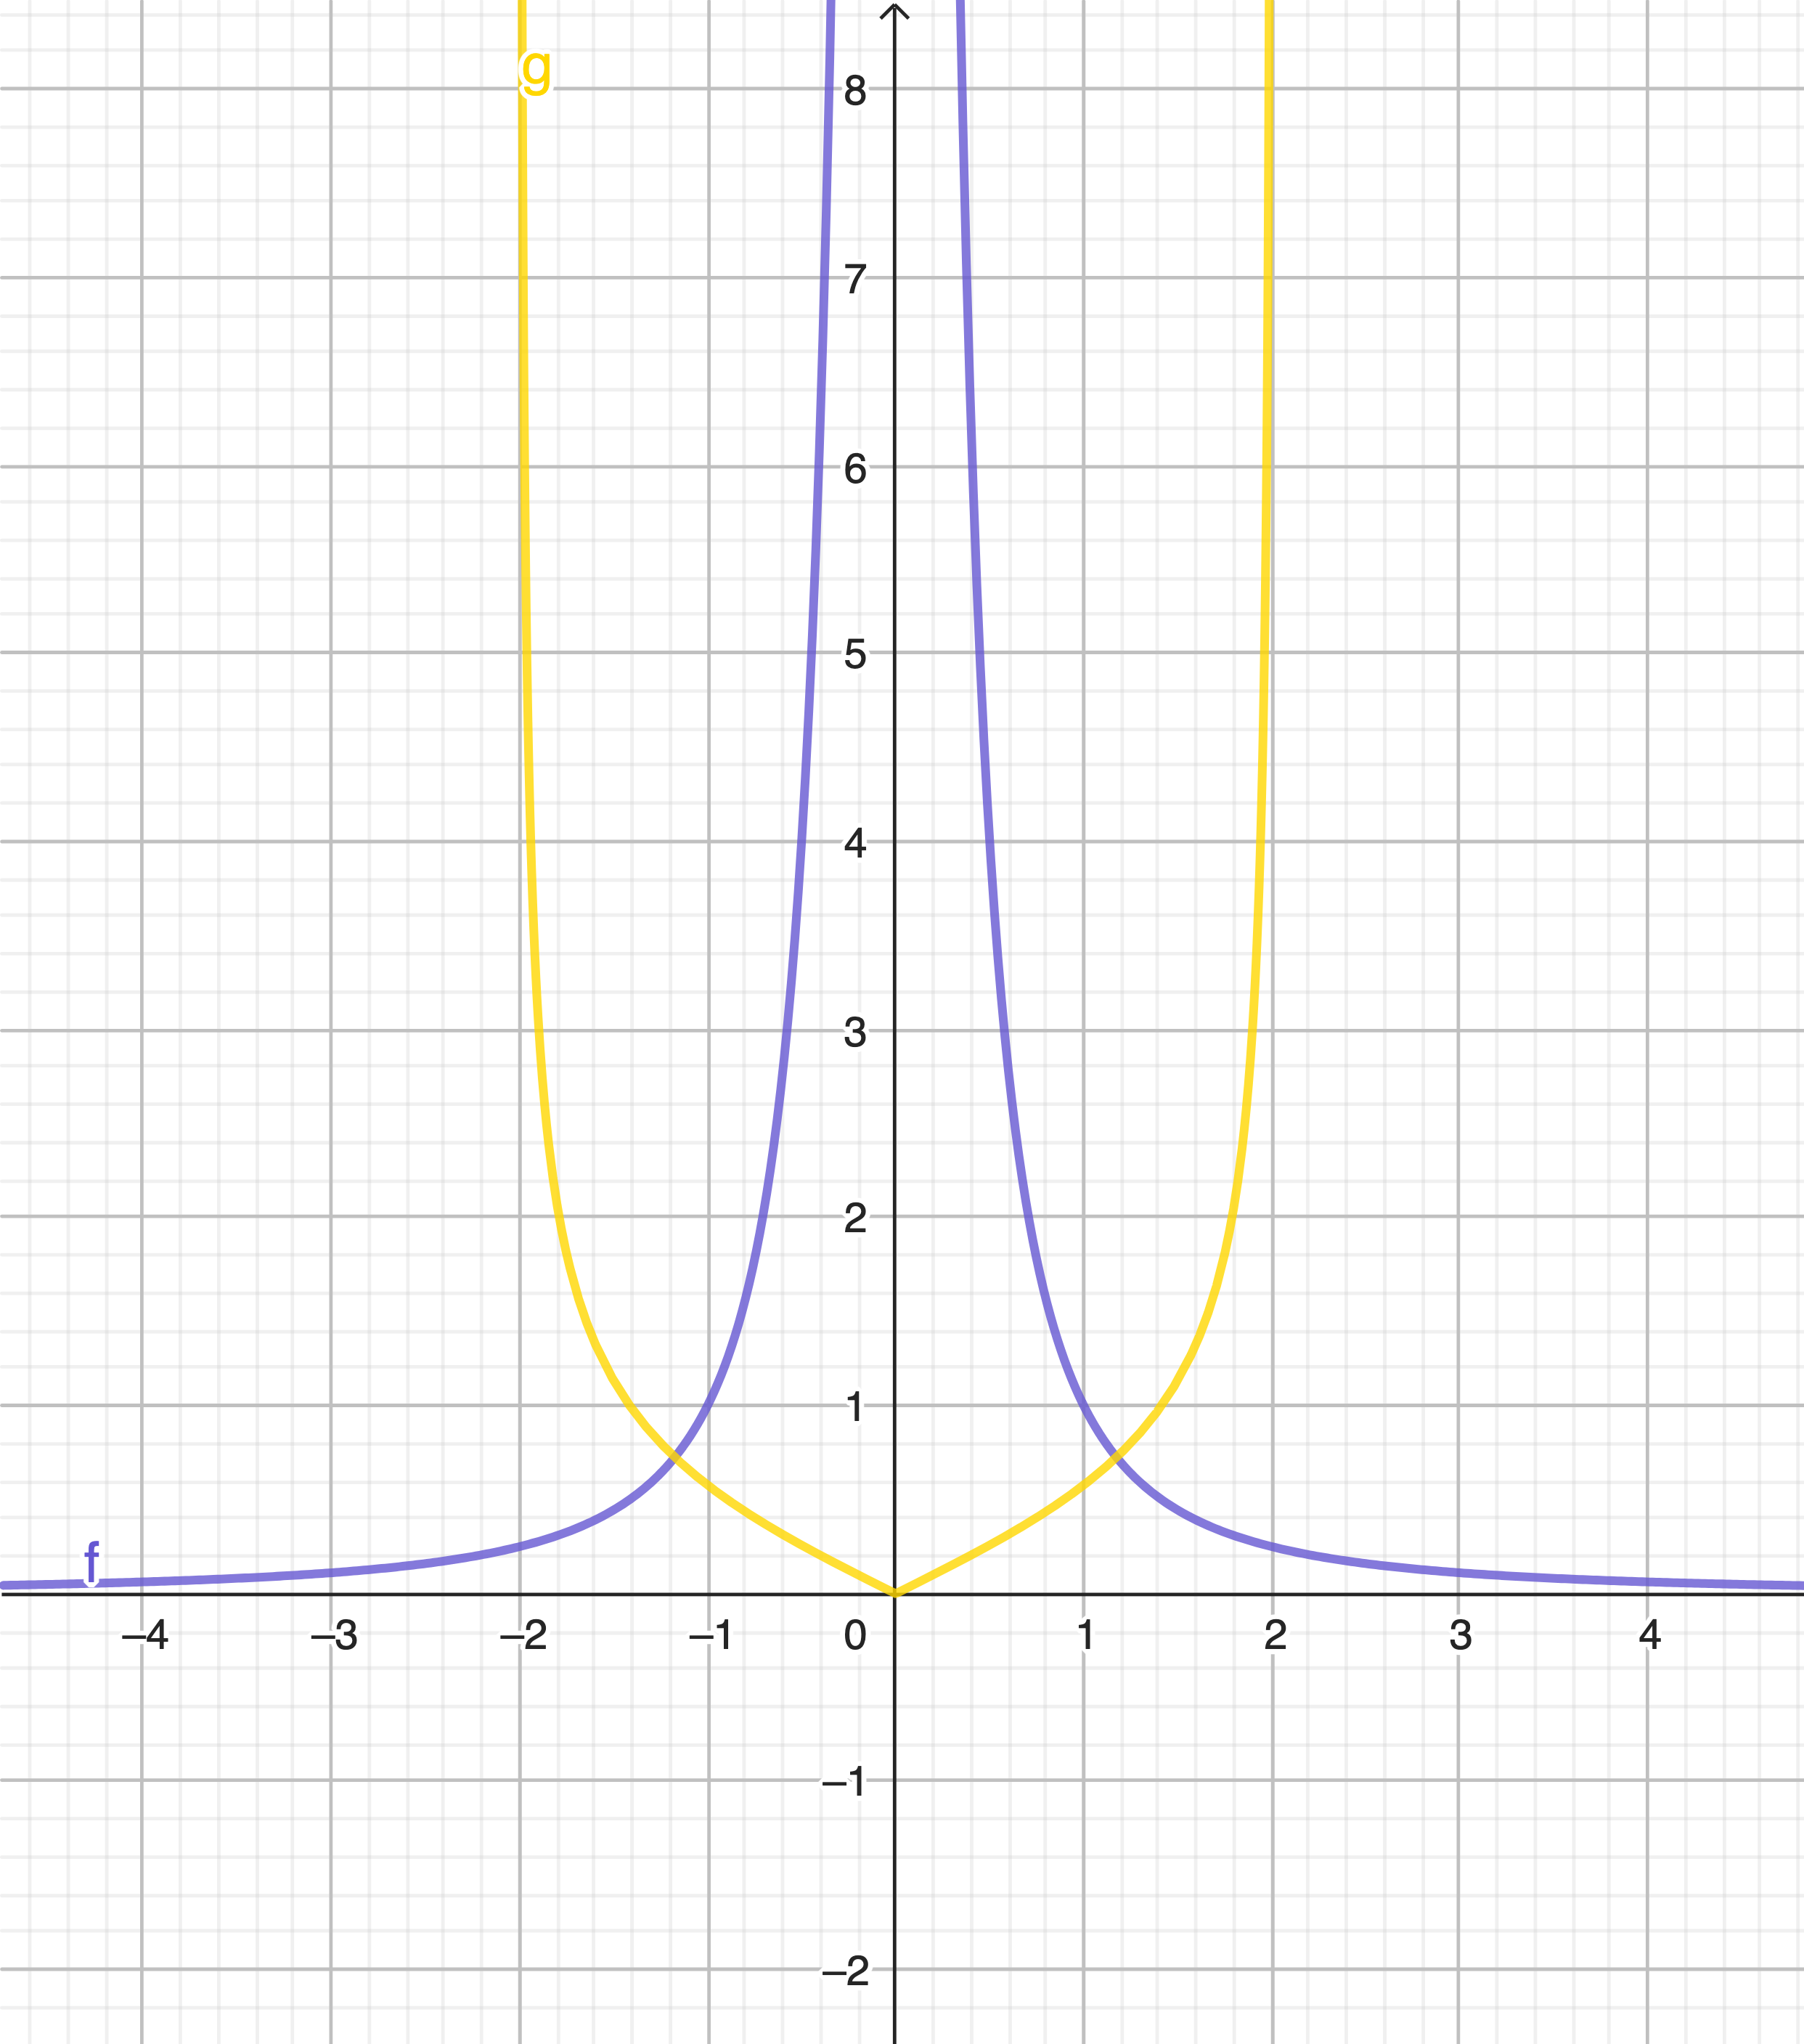
\includegraphics[width=0.6\textwidth]{images/grafico.png}
  \caption{Funzione b (viola) e a (gialla)}
  \label{fig:funzioni}
\end{figure}

%%%%%%%%%%%%%%%%%%%%%%%%%%%%%%%%%%%%%%%%%%

\section*{Pratica}
Per l'iterazione iniziale, si prende:
\[
  x^{(0)} = \begin{bmatrix} 0.1 \\ 0.5 \end{bmatrix}.
\]

La soluzione esatta del sistema, calcolata analiticamente, è:
\[
\begin{cases}
  x = \sqrt{2 + \sqrt{3}} \approx 1.93185, \\
  y = \dfrac{1}{x} \approx 0.51764.
\end{cases}
\]
L'obiettivo è verificare che il metodo converga alla soluzione.

\subsection*{Codice MATLAB per il Metodo di Approssimazione Successiva}

\begin{lstlisting}
close all
clear all
clc

%% Definizione della funzione di iterazione per il sistema
g = @(x) [sqrt(4 - x(2)^2);  % x_{n+1} = sqrt(4 - y_n^2)
          1/x(1)];           % y_{n+1} = 1/x_n

% Soluzione esatta (calcolata analiticamente)
exact_x = sqrt(2 + sqrt(3));   % ~1.93185
exact_y = 1/exact_x;           % ~0.51764
sol = [exact_x; exact_y];

% Parametri di ingresso
x0 = [0; 0.5];  % Guess iniziale vicino alla soluzione
tol = 1e-6;
maxit = 60;

% Chiamata alla funzione di punto fisso
[x, it, iterati] = fixed(g, x0, maxit, tol);

% Calcolo residuo ed errore
fprintf('Iterazioni effettuate: %d \nSoluzione: [%.12f, %.12f]\n', it, x);
for i = 1:it+1
    res(i) = norm(iterati{i} - g(iterati{i})); % Residuo
    err(i) = norm(iterati{i} - sol, inf);      % Errore assoluto
end

% Plot del residuo
figure;
semilogy(1:it+1, res, 'r*-');
title('Residuo vs Iterazioni');
xlabel('Iterazioni'); ylabel('||x_k - g(x_k)||');

% Plot dell'errore
figure;
semilogy(1:it+1, err, 'b*-');
title('Errore assoluto vs Iterazioni');
xlabel('Iterazioni'); ylabel('||x_k - x^*||_{\infty}');

% Stima dell'ordine di convergenza
[p, C] = stima_ordine(iterati); 
fprintf('Ordine stimato: %.3f \t Costante asintotica: %.3f\n', p, C);
\end{lstlisting}

\subsection*{Funzione Fixed Point}

\begin{lstlisting}
function [x,it,iterati]=fixed(g,x0,maxit,tol)
% g     funzione
% x0    punto iniziale
% maxit numero massimo di iterazioni
% tol   tolleranza relativa
%
x = x0;
iterati{1} = x;
for it = 1:maxit
    x1 = feval(g, x);
    iterati{it+1} = x1;
    if norm(x1 - x, inf) < eps + tol * norm(x, inf) % Convergenza raggiunta
        break
    end
    x = x1;  
end
end
\end{lstlisting}

\subsection*{Funzione per la Stima dell'Ordine di Convergenza}

\begin{lstlisting}
function [ordine,stima] = stima_ordine(xvect)
% Stima ordine e costante asintotica di convergenza

nit = length(xvect);
p = zeros(nit-1, 1);  % Vettore degli ordini
c = zeros(nit-1, 1);  % Vettore delle costanti

for i = 3:nit-1
    diff1 = norm(xvect{i+1} - xvect{i});
    diff2 = norm(xvect{i} - xvect{i-1});
    diff3 = norm(xvect{i-1} - xvect{i-2});

    if abs(diff1) <= eps || abs(diff2) <= eps || abs(diff3) <= eps
        p(i) = p(i-1);  % Se la precisione è troppo bassa, manteniamo il valore precedente
        c(i) = c(i-1);
    else
        num = log(diff1 / diff2);
        den = log(diff2 / diff3);
        p(i) = num / den;
        c(i) = diff1 / diff2^p(i);
    end
end
ordine = p(end);
stima = c(end);
end
\end{lstlisting}

\subsection*{Risultati da Console}

Il codice fornisce la soluzione ottenuta, il residuo e l'errore assoluto ad ogni iterazione. Ecco un esempio dei risultati:
\begin{lstlisting}[style=console]
Iterazioni effettuate: 13 	 
Soluzione: [1.931853363035, 0.517638057300]
Ordine stimato: 1.000 	 Costante asintotica: 0.268
\end{lstlisting}

Come si può notare, i risultati sono molto vicini alla soluzione analitica. Il sistema converge dopo 13 iterazioni con velocità lineare (ordine stimato = 1). Se avessimo ottenuto un ordine pari a 2, la convergenza sarebbe stata quadratica (l'errore si ridurrebbe, ad esempio, di un fattore 4 ad ogni iterazione, mentre nel caso lineare si riduce di un fattore 2).

\section*{Esercizio 2}
\textbf{Problema:} Usare il metodo di Newton per risolvere il sistema dell’esercizio precedente. Verificare sperimentalmente che, a partire dal punto \((0.5,2)\), il metodo converga localmente.

\subsection*{Metodo di Newton}
Il metodo di Newton si basa sullo sviluppo in serie di Taylor della funzione e utilizza la derivata (la Jacobiana) della funzione. In generale:
\[
  x^{(k+1)} = x^{(k)} - J(x^{(k)})^{-1} f(x^{(k)}),
\]
dove la matrice Jacobiana \( J(x) \) è definita come:
\[
	J_{ij} = \frac{\partial f_i}{\partial x_j}.
\]

Consideriamo il sistema:
\[
f(x,y)=
\begin{cases}
	x^2 + y^2 - 4,\\[1mm]
	x \cdot y - 1.
\end{cases}
\]
La Jacobiana risulta essere:
\[
J(x,y)=
\begin{pmatrix}
	2x & 2y\\[1mm]
	y & x
\end{pmatrix}.
\]

Per il punto iniziale, si prende:
\[
x^{(0)} = \begin{pmatrix} 2 \\ 0.5 \end{pmatrix}.
\]
L'obiettivo è verificare che il metodo converga alla soluzione.
Per osservare che il metodo converge dobbiamo dire
\begin{enumerate}
	\item $f$ sia di classe $C^2$
	\item Lo Jacobiano sia non degenere
\end{enumerate}
Il primo punto abbiamo già potuto verificarlo poichè abbiamo già calcolato lo Jacobiano ($J$) quindi $f\in C^1$ e continuo. Per vedere se appartiene a $C^2$ basta vedere se riusciamo a calcolarci lo Jacobiano di $J$ che sarebbe:
\[
\begin{matrix}
	\frac{\partial^2 f_1}{\partial x^2}=2 & \frac{\partial^2 f_1}{\partial y^2}=2 & \frac{\partial^2 f_2}{\partial x \partial y}=1
\end{matrix}
\]
\[
J''=
\begin{bmatrix}
	2&2\\
	1&1\\
\end{bmatrix}
\]
Sono tutte costanti, tutte continue quindi $f \in C^2$\\
Per risolvere il secondo punto dobbiamo quando  lo Jacobiano ($J$) è invertibile. Calcoliamo il determinante se questo è diverso da 0 allora è invertibile.
\[
\begin{align}
	det(J)&=2x*x-2y*y\neq0\\
	&=2(x-y)(x+y)\neq 0
\end{matrix}
\]
Il tutto ha risoluzione a:
\[
\begin{align}
	x&=y\\
	x&=-y
\end{matrix}
\]
Quindi il mio sistema non converge quando la mia x è uguale alla mia y e quando è il contrario della mia y. Quindi nel caso della mia $x^0$ ho convergenza.

\begin{figure}[H]
  \centering
  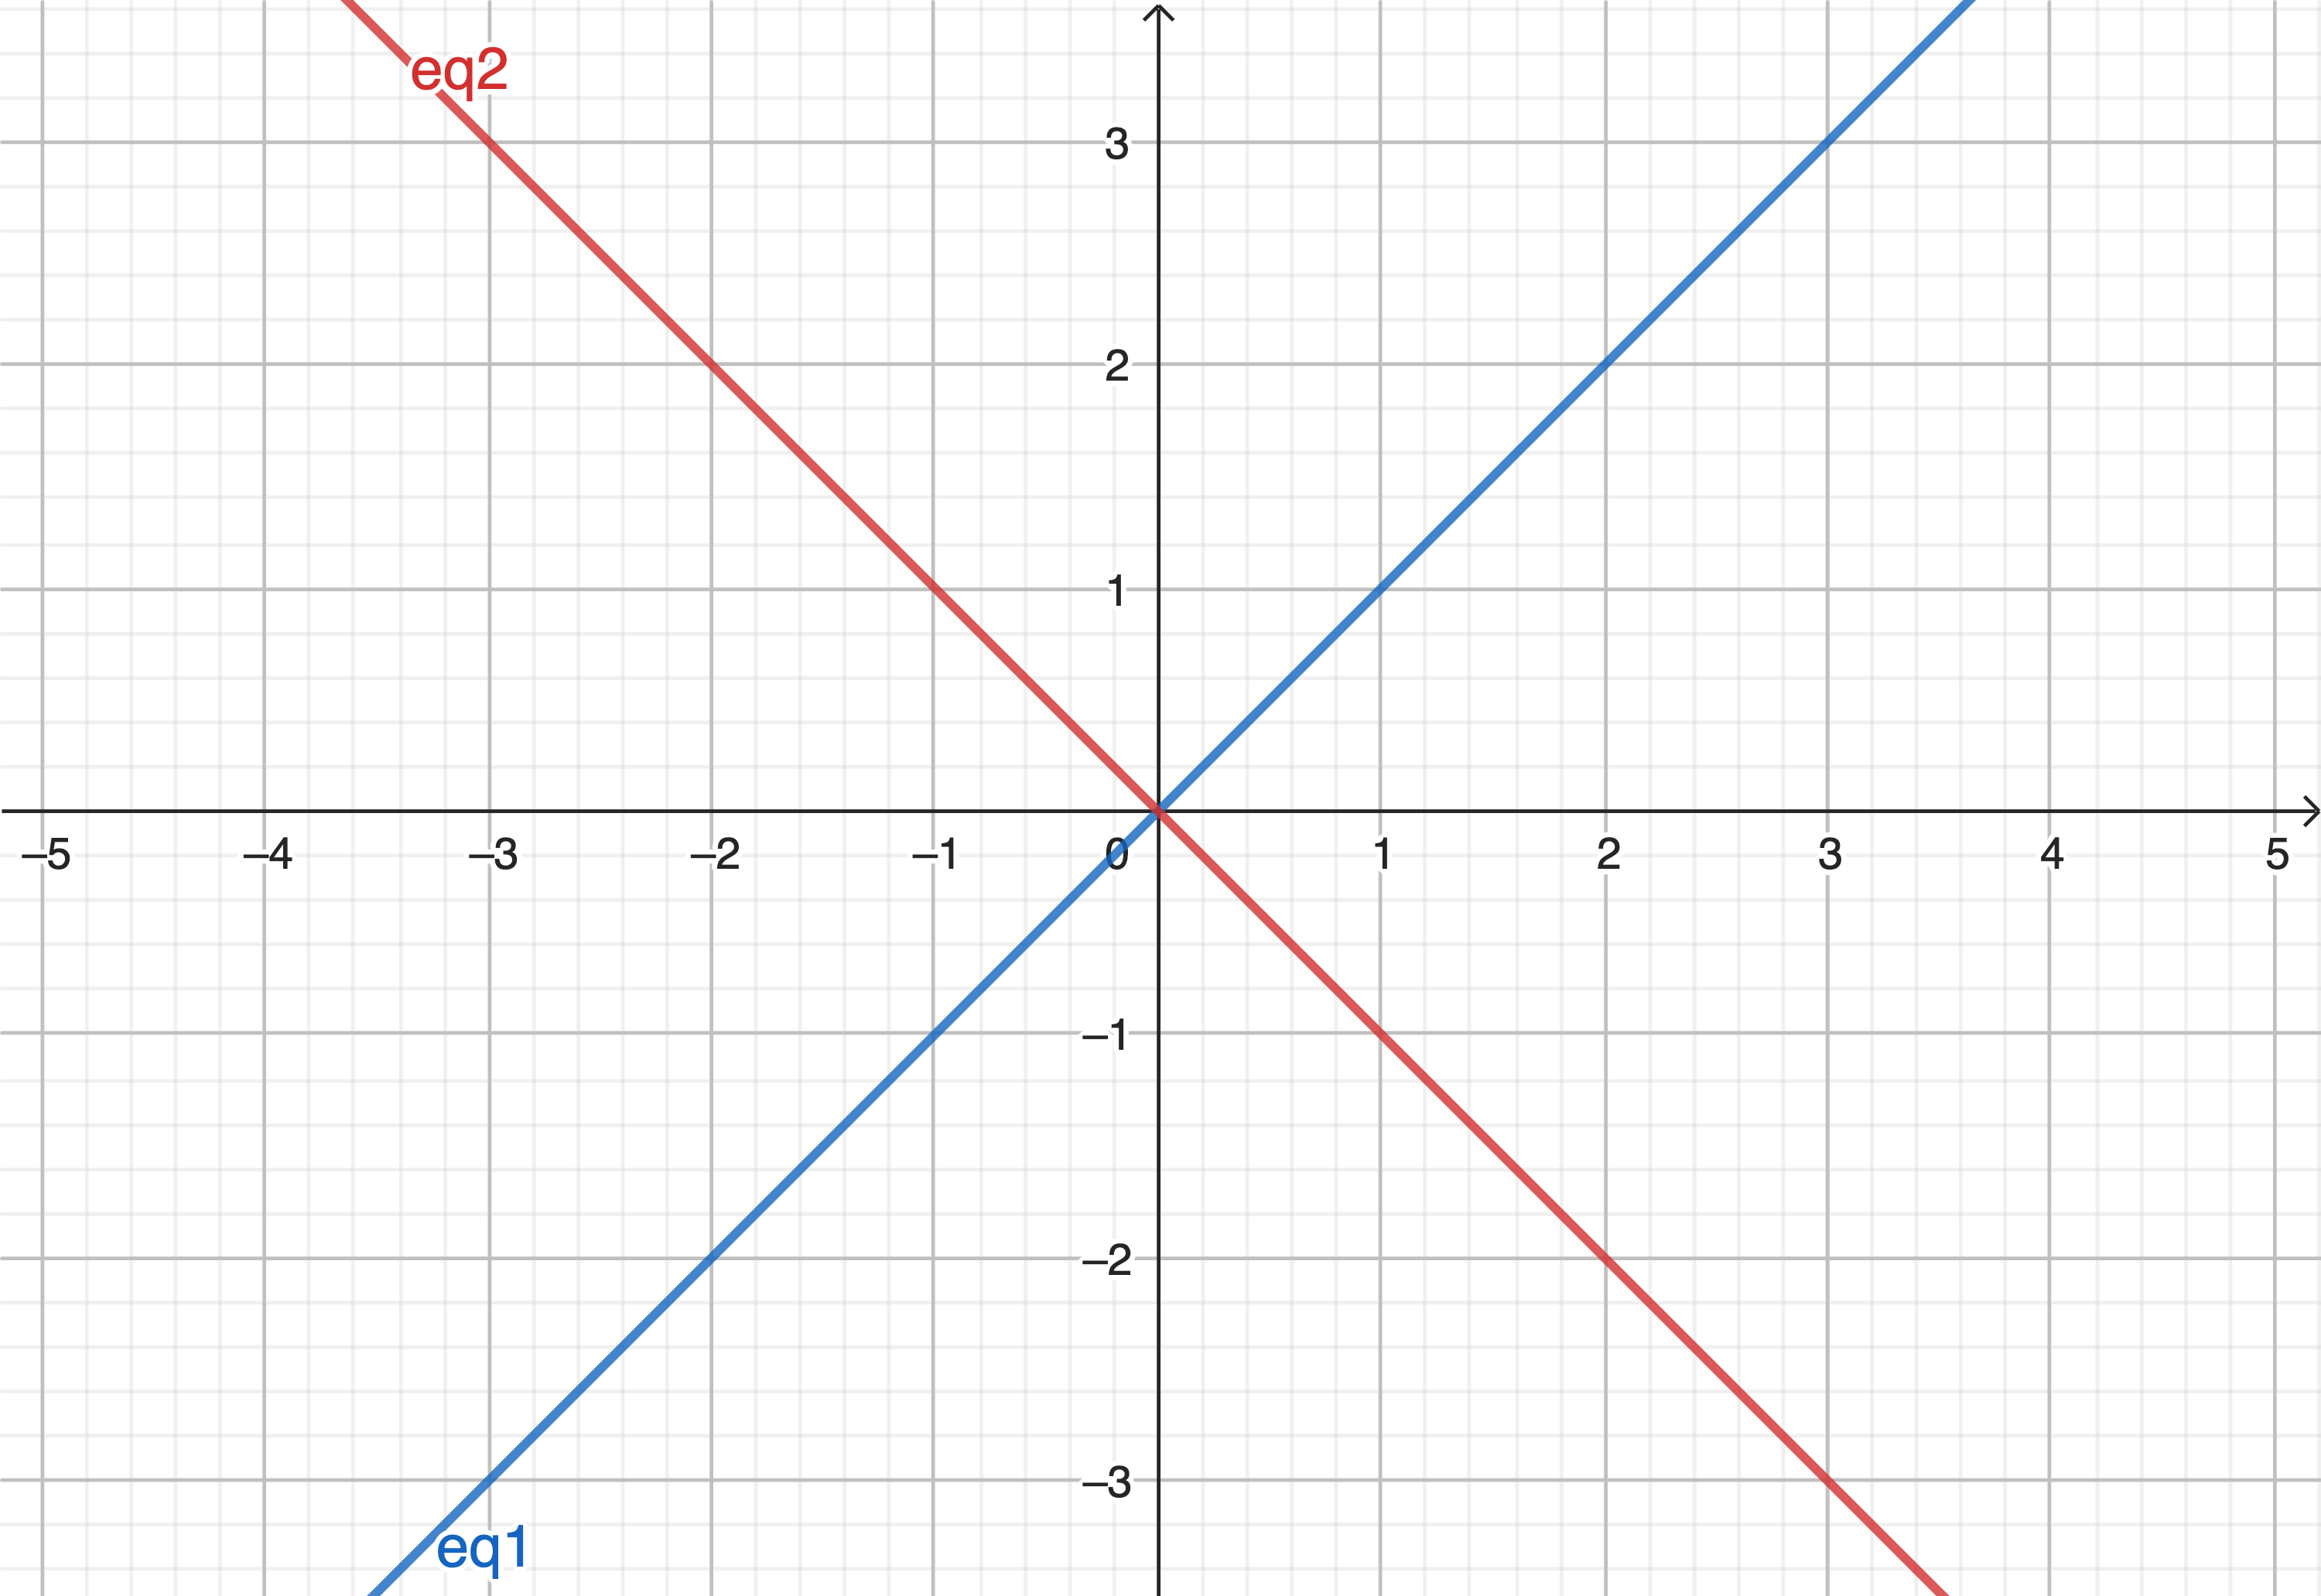
\includegraphics[width=0.7\textwidth]{images/exist.png} 
  \caption{Valori per cui non converge il sistema}
  \label{fig:esiste?}
\end{figure}


\subsection*{Codice MATLAB per il Metodo di Newton}

\begin{lstlisting}
close all
clear all
clc

%% Definizione della funzione f e della sua Jacobiana J
f = @(x) [x(1)^2 + x(2)^2 - 4;
          x(1)*x(2) - 1];

J = @(x) [2*x(1), 2*x(2);
          x(2),   x(1)];

% Soluzione esatta (calcolata analiticamente)
exact_x = sqrt(2 + sqrt(3));   % ~1.93185
exact_y = 1/exact_x;           % ~0.51764
sol = [exact_x; exact_y];

% Parametri di ingresso
x0 = [2; 0.5];  % Guess iniziale dato dalla consegna del problema
tolx = 1e-6; tolf = 1e-6;
maxit = 60;

% Chiamata alla funzione Newton
[x, it, iterati] = sis_newton(f, J, x0, tolx, tolf, maxit);

% Calcolo residuo ed errore
fprintf('Iterazioni effettuate: %d \t Soluzione: [%.12f, %.12f]\n', it, x);
for i = 1:it+1
    res(i) = norm(iterati{i} - f(iterati{i})); % Residuo
    err(i) = norm(iterati{i} - sol, inf);      % Errore assoluto
end

% Plot residuo
figure;
semilogy(1:it+1, res, 'r*-');
title('Residuo vs Iterazioni');
xlabel('Iterazioni'); ylabel('||f(x_k)||');

% Plot errore
figure;
semilogy(1:it+1, err, 'b*-');
title('Errore assoluto vs Iterazioni');
xlabel('Iterazioni'); ylabel('||x_k - x^*||_{\infty}');

% Stima ordine di convergenza
[p, C] = stima_ordine(iterati); 
fprintf('Ordine stimato: %.3f \t Costante asintotica: %.3f\n', p, C);
\end{lstlisting}

\subsection*{Funzione Newton}

\begin{lstlisting}
function [x, it, iterati] = sis_newton(fvett, jac, x0, tolx, tolf, maxit)
    x = x0(:);
    iterati{1} = x;
    f_val = feval(fvett, x);
    J_val = feval(jac, x);
    for it = 1:maxit
        dx = J_val \ (-f_val);  % Calcolo dell'incremento
        x = x + dx;
        f_val = feval(fvett, x);
        iterati{it+1} = x;
        if (norm(dx, inf) <= eps + tolx * norm(x, inf)) && (norm(f_val, inf) <= tolf)
            break
        end
        J_val = feval(jac, x);
    end
    if it >= maxit
        fprintf('Raggiunto il massimo numero di iterazioni\n');
    end
end
\end{lstlisting}

\subsection*{Risultati da Console}

Esempio di output ottenuto dalla console:
\begin{lstlisting}[style=console]
Iterazioni effettuate: 3 	 
Soluzione: [1.931851652579, 0.517638090204]
Ordine stimato: 1.933 	 Costante asintotica: 0.313
\end{lstlisting}

Si osserva che il metodo di Newton converge in sole 3 iterazioni e, contrariamente al metodo delle approssimazioni successive, mostra una convergenza di ordine quadratico (il che implica una riduzione dell'errore molto più rapida ad ogni iterazione).

\section*{Differenza tra Es1 e Es2}
Poniamo che entrambi gli esercizi utilizzino le stesse coordinate iniziali
\[
x_0=\begin{pmatrix} 2 \\ 0.5 \end{pmatrix}
\]
e che le tolleranze siano uguali. Di seguito si riportano i risultati grafici.

\begin{figure}[H]
  \centering
  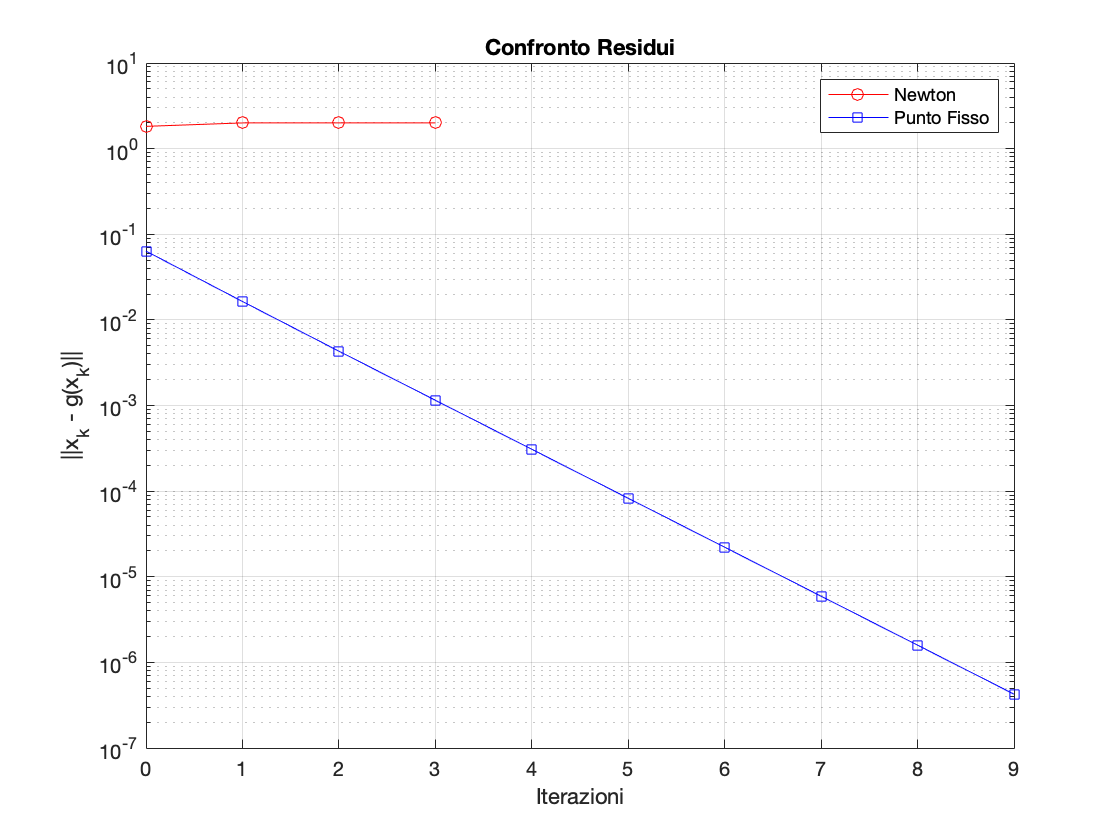
\includegraphics[width=0.7\textwidth]{images/figure1.png} 
  \caption{Confronto dei residui per iterazioni}
  \label{fig:residui}
\end{figure}

Nella figura si osserva come il residuo vari in funzione delle iterazioni. In particolare, il metodo delle approssimazioni successive, pur raggiungendo un residuo minore, richiede un numero maggiore di iterazioni rispetto al metodo di Newton. Quest'ultimo, infatti, converge in 3 iterazioni, mentre il primo impiega circa 9 iterazioni.

\begin{mdframed}[linecolor=blue, linewidth=1pt, roundcorner=10pt]
\paragraph{Esempio Pratico}
Il residuo associato a un sistema lineare \(A\mathbf{x} = \mathbf{b}\) è definito come:
\[
\mathbf{r} = \mathbf{b} - A\mathbf{x},
\]
che rappresenta la differenza tra il termine noto \(\mathbf{b}\) e la stima \(A\mathbf{x}\).
\end{mdframed}

\begin{figure}[H]
  \centering
  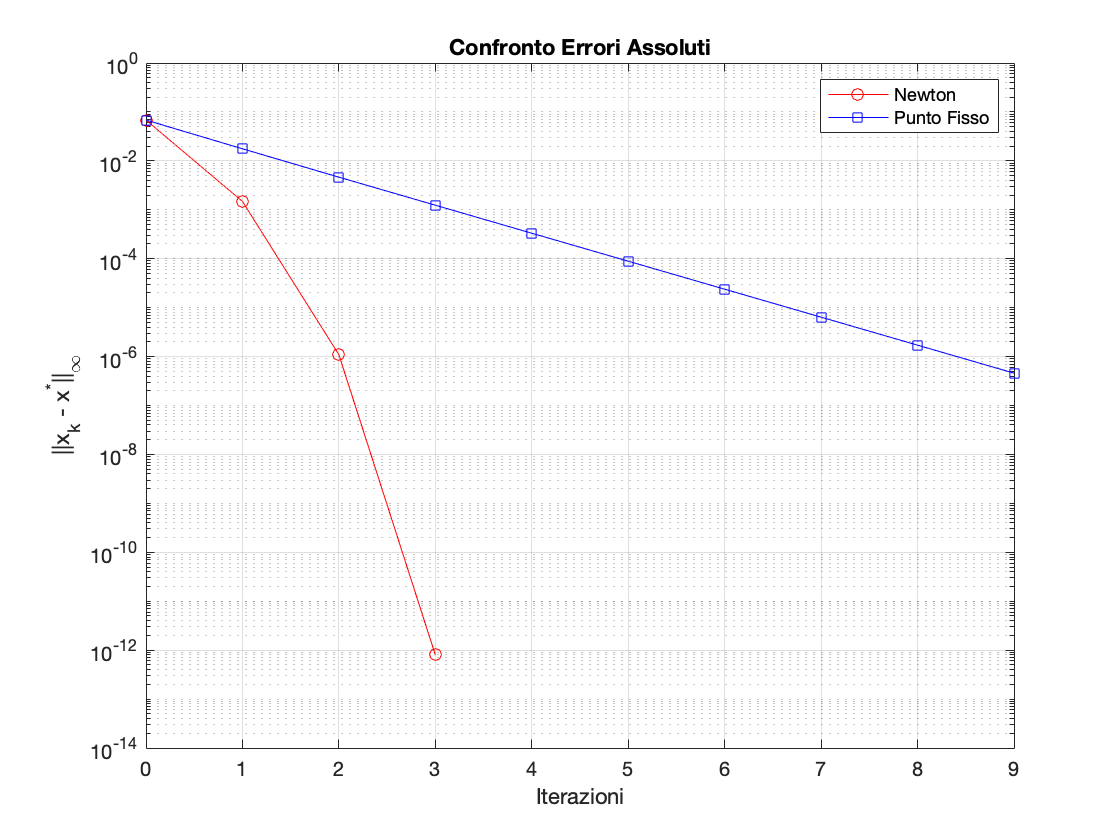
\includegraphics[width=0.7\textwidth]{images/figure2.png} 
  \caption{Confronto degli errori assoluti per iterazioni}
  \label{fig:errore}
\end{figure}
Nel grafico degli errori, si nota come l'errore assoluto nel metodo delle approssimazioni successive sia maggiore rispetto a quello ottenuto con il metodo di Newton, che raggiunge valori prossimi alla tolleranza impostata.

\begin{lstlisting}[style=console]
============= RISULTATI =============
Newton: Ordine 1.933 - Costante 0.313
Punto Fisso: Ordine 1.000 - Costante 0.268	
\end{lstlisting}
Come evidenziato, la velocità di convergenza (cioè la rapidità con cui l'errore si riduce ad ogni iterazione) è significativamente maggiore per il metodo di Newton, confermando la convergenza quadratica rispetto alla convergenza lineare del metodo delle approssimazioni successive.




%%%%%%%%%%%%%%%%%%%%%%%%%%%%%%%%%%%%%%%%%%




%%%%%%%%%%%%%%%%%%%%%%%%%%%%%%%%%%%%%%%%%%
\section*{Esercizio 3 (Aereo)}
%%%%%%%%%%%%%%%%%%%%%%%%%%%%%%%%%%%%%%%%%%

\subsection*{Descrizione del Problema}
Si consideri un modello semplificato di controllo della stabilità di un aereo in risposta ai comandi del pilota, basato su equazioni di bilanciamento delle forze, in cui il termine di gravità è ignorato. In particolare, il sistema è formato da 5 equazioni in 8 incognite e si esprime come
\[
A x + \psi(x) = 0,
\]
dove
\[
A =
\begin{pmatrix}
-3.933 & 0.107 & 0.126 & 0     & -9.99  & 0      & -45.83 & -7.64 \\
0      & -0.987& 0     & -22.95& 9      & -28.37& 0      & 0     \\
0.002  & 0     & -0.235& 0     & 5.67   & 0      & -0.921 & -6.51 \\
0      & 1.0   & 0     & -1.0  & 0      & -0.168& 0      & 0     \\
0      & 0     & -1.0  & 0     & -0.196 & 0      & -0.0071& 0
\end{pmatrix}
\]
e
\[
\psi(x)=
\begin{pmatrix}
-0.727\,x_2x_3 + 8.39\,x_3x_4 - 684.4\,x_4x_5 + 63.5\,x_4x_2 \\
0.949\,x_1x_3 + 0.173\,x_1x_5 \\
-0.716\,x_1x_2 - 1.578\,x_1x_4 + 1.132\,x_4x_2 \\
-x_1x_5 \\
x_1x_4
\end{pmatrix}.
\]
Le variabili \(x_1\), \(x_2\) e \(x_3\) rappresentano, rispettivamente, le velocità di rollio, beccheggio e imbardata, mentre \(x_4\) e \(x_5\) sono gli angoli di attacco e di derapata. Le ultime tre incognite \(x_6\), \(x_7\) e \(x_8\) rappresentano i controlli (deviazione di elevatore, alettone, timone).

Per studiare il comportamento dell’aereo al variare dei controlli, si fissa il vettore \( u\in\mathbb{R}^3 \) (i comandi del pilota) e si risolve il sistema ridotto di 5 equazioni in 5 incognite. In particolare, ponendo
\[
A = [A_1 \quad A_2],\quad A_1\in\mathbb{R}^{5\times5},\quad A_2\in\mathbb{R}^{5\times3},
\]
si scrive la variabile
\[
x = \begin{pmatrix} w \\ u \end{pmatrix},\quad \text{con } w\in\mathbb{R}^5 \text{ e } u\in\mathbb{R}^3.
\]
Fissato \(u\), siccome \(A_1\) è non singolare, il sistema diventa:
\[
A_1 w + A_2 u + \psi(w) = 0,
\]
ovvero, applicando l'inverso di \(A_1\),
\[
w = - A_1^{-1}\Bigl(A_2 u + \psi(w)\Bigr).
\]
In questo modo vale, formalmente, anche
\[
\varphi(x) = A_1^{-1}.
\]

\vspace{1em}
\subsection*{Obiettivo e Considerazioni sull'Implementazione in MATLAB}
Per rendere l'esercizio più completo e "carino", nel codice MATLAB sono stati integrati:

\begin{itemize}
  \item Un timer che misura il tempo di esecuzione per ciascun metodo;
  \item Due metodi di risoluzione: una risoluzione per sistema (basata sulla riscrittura della matrice) e una risoluzione con il metodo delle approssimazioni successive (usando \texttt{feval}).
\end{itemize}

Si sono inoltre sperimentate varianti per il metodo di Newton (Newton Globale) ma, a causa della complessità della Jacobiana del sistema, si è preferito evitare tale approccio per questo esercizio.

\vspace{1em}
I dati iniziali sono:
\[
x_0=\begin{bmatrix}0\\0\end{bmatrix}
\quad \text{e} \quad
u = \begin{bmatrix}0.1\\0.1\\0.1\end{bmatrix},
\]
dove \(u\) rappresenta i comandi del pilota (valori compresi fra 0 e 1 nelle direzioni x, y, z dello spazio).

%%%%%%%%%%%%%%%%%%%%%%%%%%%%%%%%%%%%%%%%%%
\subsection*{Codice MATLAB per il Metodo delle Approssimazioni Successive}
%%%%%%%%%%%%%%%%%%%%%%%%%%%%%%%%%%%%%%%%%%

Di seguito viene riportato il codice MATLAB utilizzato per risolvere il problema dell'aereo:

\begin{lstlisting}
close all
clear all
clc
addpath("/Users/tobiasacchetto/Documents/GitHub/Numerical_Analysis_II/Function");

% Definizione della matrice A
A = [ -3.933  0.107   0.126   0   -9.99   0   -45.83  -7.64;
       0      -0.987   0    -22.95   9    -28.37   0       0;
       0.002   0      -0.235   0    5.67    0    -0.921  -6.51;
       0       1.0     0    -1.0     0    -0.168   0       0;
       0       0      -1.0    0    -0.196   0    -0.0071  0];

% Partitione della matrice A in A1 e A2
A1 = A(1:5,1:5);
A2 = A(1:5,6:8);

% Definizione della funzione non lineare psi(w)
psi = @(w) [ -0.727*w(2)*w(3) + 8.39*w(3)*w(4) - 684.4*w(4)*w(5) + 63.5*w(4)*w(2);
             0.949*w(1)*w(3) + 0.173*w(1)*w(5);
            -0.716*w(1)*w(2) - 1.578*w(1)*w(4) + 1.132*w(4)*w(2);
            -w(1)*w(5);
             w(1)*w(4) ];

% Vettore dei controlli (u) e stato iniziale per w
u = [0.1; 0.1; 0.1];  % [x6; x7; x8]
w_old = zeros(5, 1);

% Parametri iterativi
max_iter = 100;
tolerance = 1e-6;

tic;
% Iterazione del punto fisso: A1*w^(k+1) = -(A2*u + psi(w^(k)))
for iter = 1:max_iter
    psi_w = psi(w_old);
    rhs = A2 * u + psi_w;
    w_new = - (A1 \ rhs);
    
    if norm(w_new - w_old) < tolerance
        fprintf('Convergenza raggiunta in %d iterazioni.\n', iter);
        break;
    end
    w_old = w_new;
end
tempo = toc;
% Output del risultato
disp('Computed state vector w:');
disp(w_new);
fprintf('Il tempo impiegato è %g sec.\n\n', tempo);

% Alternativamente, uso la funzione "fixed" basata su feval
f = @(x)(-inv(A1)*(A2*u + psi(x)));
tic;
[x, it, iterati] = fixed(f, w_old, max_iter, tolerance);
tempo = toc;
disp('Computed state vector w:');
disp(x);
fprintf('Numero di iterazioni: %d\n', it);
fprintf('Il tempo impiegato è %g sec.\n\n', tempo);
\end{lstlisting}

%%%%%%%%%%%%%%%%%%%%%%%%%%%%%%%%%%%%%%%%%%
\subsection*{Risultati da Console}
%%%%%%%%%%%%%%%%%%%%%%%%%%%%%%%%%%%%%%%%%%
\begin{lstlisting}[style=console]
Convergenza raggiunta in 14 iterazioni.
Computed state vector w:
   -0.0363
   -0.0580
   -0.0237
   -0.0700
    0.1303

Il tempo impiegato è 0.00674418 sec.

Computed state vector w:
   -0.0363
   -0.0580
   -0.0237
   -0.0700
    0.1303

Numero di iterazioni: 3
Il tempo impiegato è 0.00463188 sec.
\end{lstlisting}

\vspace{1em}
\textbf{Considerazioni Finali:}  
Si osserva che, nel primo caso (risoluzione tramite la messa a sistema delle matrici), la convergenza viene raggiunta dopo 14 iterazioni, mentre nel secondo (utilizzando \texttt{feval} nel metodo delle approssimazioni successive) il risultato si ottiene in sole 3 iterazioni, con una marcata differenza nel tempo di esecuzione. Tuttavia, il sistema risulta instabile: se in input il vettore \(u\) assume valori superiori a 0.16 per una qualsiasi delle componenti, il sistema non converge (vengono restituiti NaN).

\vspace{1em}
Successivamente viene sperimentato un approccio con Newton Globale per migliorare la stabilità, ma il metodo, pur essendo implementato con un timer e con il calcolo della Jacobiana, non converge poiché la procedura entra in un minimo locale. Di seguito si riporta la parte di codice per il metodo Newton Globale:

\begin{lstlisting}
close all
clear all
clc
addpath("/Users/tobiasacchetto/Documents/GitHub/Numerical_Analysis_II/Function");

% Definizione della matrice A
A= [
    -3.933 0.107 0.126 0 -9.99 0 -45.83 -7.64;
    0 -0.987 0 -22.95 9 -28.37 0 0;
    0.002 0 -0.235 0 5.67 0 -0.921 -6.51;
    0 1.0 0 -1.0 0 -0.168 0 0;
    0 0 -1.0 0 -0.196 0 -0.0071 0;
    ];
A1=A(1:5,1:5);
A2=A(1:5,6:8);

psi = @(w) [ -0.727*w(2)*w(3) + 8.39*w(3)*w(4) - 684.4*w(4)*w(5) + 63.5*w(4)*w(2);
             0.949*w(1)*w(3) + 0.173*w(1)*w(5);
            -0.716*w(1)*w(2) - 1.578*w(1)*w(4) + 1.132*w(4)*w(2);
            -w(1)*w(5);
             w(1)*w(4) ]; 

% Impostazione dei controlli e punto iniziale per w
u = [0.6; 0.1; 0.1];  % [x6; x7; x8]
x0 = [0.1; 0.1; 0.1; 0.1; 0.1];

max_iter = 150;
tolerance = 1e-6;
f = @(x)(-A1\(A2*u+psi(x)));

% Definizione della Jacobiana in forma di function handle (già sintetizzata)
J = @(w) [ -3933/1000, (127*w(4))/2 - (727*w(3))/1000 + 107/1000, (839*w(4))/100 - (727*w(2))/1000 + 63/500, (127*w(2))/2 + (839*w(3))/100 - (3422*w(5))/5, - (3422*w(4))/5 - 999/100;
           (949*w(3))/1000 + (173*w(5))/1000, -987/1000, (949*w(1))/1000, -459/20, (173*w(1))/1000 + 9;
           1/500 - (789*w(4))/500 - (179*w(2))/250, (283*w(4))/250 - (179*w(1))/250, -47/200, (283*w(2))/250 - (789*w(1))/500, 567/100;
           -w(5), 1, 0, -1, -w(1);
           w(4), 0, -1, w(1), -49/250 ];

tolx = tolerance;
tolf = tolerance;
[x, it, iterati, merito] = sis_newton_glob(f, J, x0, tolx, tolf, max_iter);
disp('Computed state vector w:');
disp(x);
fprintf('Numero di iterazioni: %d\n', it);
% L'algoritmo non converge in quanto, ad un certo punto, Newton Globale entra in un minimo locale.
\end{lstlisting}

\vspace{1em}
\textbf{Risultati (Newton Globale):}

\begin{lstlisting}[style=console]
raggiunto massimo numero di iterazioni
Computed state vector w:
    0.3123
    1.6668
    0.5181
    0.0029
    0.1536

Numero di iterazioni: 150
\end{lstlisting}
Come evidenziato, indipendentemente dal numero di iterazioni, Newton Globale non riesce a convergere: dopo un certo punto il metodo entra in un minimo locale, correggendo continuamente senza ridurre significativamente l'errore.

\end{document}